\section{Controlled transfer from the same failure history}
\label{sec:c24}
The earlier comparison re-formed a local method within each task group. It did
not test a single frozen method transported to new timing mechanisms. The older
waveform study also left a concrete ambiguity: successful designs used a
0.75 s sampling period, but a fixed-method control did so as well
(Appendix~\ref{sec:lineages}). Remembering that value cannot establish a general
relation among sampling, confirmation, timestamp origin and allowed error.
C24 therefore tests frozen method transfer with an explicit equal-history
control. Its prespecified falsifier is no gain against that control; the observed
result meets this falsifier for an improvement claim.

\subsection{A timing component with independently checked service}
This new component intentionally isolates time semantics under ideal continuous
power and a fixed link delay. It does not rerun or qualify the original O
energy, RF or keepalive service. The fixed waveform defines continuous threshold
excursions. An event qualifies only after its required confirmation duration;
the task then defines its true timestamp as either excursion onset or
qualification time. At each scheduled poll, the program first confirms the
previously held observation and then applies the new sample. The program never
reads the reference event list or acceptance verdict.

Legal $D$ fields are sampling period, sampling phase, timestamp origin, and a
constant timestamp offset. Origins are the confirmation poll, first qualifying
sample, or the midpoint between that sample and its preceding scheduled sample.
The fixed clock law applies signed constant drift, followed by nearest-grid
timestamp rounding and the existing millisecond frame encoding. Reception is
detection time plus the fixed 70 ms link delay. Event matching, timely reception,
and timestamp accuracy are independently checked; passing only one gate is not
complete service. In particular, timely delivery can carry a wrong event time.

\begin{table}[htbp]
\centering\small
\begin{tabular}{@{}llrrrr@{}}
\toprule
Task & Event time & Start/stop confirm. (s) & Quantum (ms) & Tolerance (ms) & Clock (ppm) \\
\midrule
Phase & Qualification & 3.00 / 4.00 & 20 & 130 & $+150$ \\
Confirmation & Qualification & 1.37 / 2.83 & 80 & 180 & $-250$ \\
Definition & Onset & 1.90 / 3.10 & 200 & 160 & $+300$ \\
\bottomrule
\end{tabular}
\caption{The three frozen formal timing conditions. Waveform transitions are
off-grid; the task JSON also fixes the source waveform and 6.5 s matching and
delivery windows. These are three within-model task conditions, not independent
hardware families.}\label{tab:ctasks}
\end{table}

\subsection{Formation, freezing, and exposure controls}
The four arms are unchanged $H_0$ with the task and public apparatus; unchanged
$H_0$ plus the original failure history; ordinary reflection from that history;
and the proposed typed timing procedure from the same history. The last three
receive identical historical information and source/tool permissions. Ordinary
reflection has access to the same executable relation language as the proposed
arm. Thus the comparison does not give one learned method an interpreter that
its control lacks. The task facts and legal design tools are common to all four.

Each reflection arm has exactly one actual model-authored formation and one
independent validation episode. Formation sees the retained original O failures,
not the new validation, first-use or final task inputs. Codex supplies task
mechanisms, a generic expression interpreter and independent evaluation; it does
not supply the learned equation. A method submission contains hypothesis,
falsifier, method text and up to eight named Boolean expression trees. The
interpreter permits fixed arithmetic, comparison and logic operators with
declared timing variables; it accepts no executable source code. Structural
admission means this artifact can be consumed, not that its claims are true.

Both structurally admitted original methods are frozen and carried unchanged
through validation and final use, including false relation returns. Validation
does not select the better method or authorize rewriting a failed clause. The
proposed arm also receives one separately identified first-use task; that result
is excluded from the final 24-attempt denominator. No new method is formed from
that success. There is one $H$ formation per reflection arm, not six independent
formations or a new $G$ lineage experiment.

The finite final list is three conditions times four arms times two fresh
contexts. Each solver entry permits at most 12 model requests, 900 s, 40 tool
calls and two distinct designs, with no automatic retry. Ordinary and proposed
formation use the same admitted limits and one-submission rule. The common
65,536-token output ceiling was frozen before the new batch. It does not replace
or reclassify the four older 32,768-token-censored attempts.

The sealed input audit checks 48 actual initial API payloads and 129 bound source
files across ABC, verifies within-task input parity and the shared history's
semantic identity, and reports only the model alias \texttt{deepseek-flash}.
Underlying model weights/version remain UNKNOWN. C-specific final references
bind all 24 episode-result byte hashes and both original method files. These
saved-data checks add no model request or scientific execution.

\subsection{The learned relations are hypotheses with a domain}
The ordinary method proposes a centered sampling budget that adds half a sample
period, half the timestamp quantum, definition delay, clock-error bound and link
delay. It also prescribes an origin-dependent offset. The proposed method
separates confirmation-grid alignment, origin/clock/rounding error,
sub-confirmation excursions, and delivery delay. In its qualified-event domain,
its origin budget has the form
\begin{equation}
 B_H=\frac{p}{2}+|\delta-c(o)|+e_{\rm clock}+\frac{q}{2}
 \;\leq\;\epsilon,
 \label{eq:learned}
\end{equation}
where $p$ is sample period, $\delta$ the offset, $o$ the timestamp origin,
$q$ the quantum and $\epsilon$ the task tolerance. Its stated centers are
$c(\mathrm{detected})=-p/2$, $c(\mathrm{midpoint})=0$, and
$c(\mathrm{first})=C-p/2$, where $C$ is confirmation duration. Equation~\ref{eq:learned}
reports the frozen model hypothesis, not a theorem established by this study.
The proposed artifact explicitly requires qualification-time semantics; the
onset task can therefore lie outside this relation's asserted domain.

The proposed sub-confirmation check instantiates the largest short excursion as
$d_{\rm short}=0.75C$, inherited from the original history. That ratio is not a
universal law of future waveforms. A syntactically general variable expression
can retain a history-specific premise. Neither artifact is hand-edited to make
its relations agree with final outcomes.

\subsection{All four arms succeed; the equal-history control is cheaper}
\begin{table}[htbp]
\centering\small
\begin{tabular}{@{}lrrrr@{}}
\toprule
Arm & Service PASS & Requests & USD upper & $H$ false on PASS \\
\midrule
Fixed $H_0$ & 6/6 & 28 & 0.1815672 & --- \\
$H_0$ + history & 6/6 & 26 & 0.6988500 & --- \\
Ordinary reflection & 6/6 & 43 & 1.1057187 & 6/6 \\
Proposed method & 6/6 & 29 & 0.7532616 & 2/6 \\
\bottomrule
\end{tabular}
\caption{C24 formal transfer: three task conditions times two fresh contexts per arm. Every design passes event matching, timely reception and timestamp accuracy. The last column counts successful designs with at least one frozen relation returning false; it is not an error rate or a proof of unsoundness. The fixed controls submit no learned relation set. Costs here exclude the separately listed formation, validation and first-use stages.}\label{tab:cformal}
\end{table}

All 24 submitted final designs pass every time-component gate, with no wrong
service judgment, incomplete entry or token-censored entry in this new list.
The proposed arm uses 29 requests and USD 0.7532616 upper, versus 26 and
USD 0.6988500 for unchanged $H_0$ with the same history. It therefore adds no
success and uses three more requests and USD 0.0544116 more even before charging
formation and validation. Ordinary reflection uses 43 requests and
USD 1.1057187. The task-only $H_0$ also succeeds 6/6, at 28 requests and
USD 0.1815672. History exposure and token length make this last comparison
different from the equal-history contrast; request count and token charge are
separate cost measures.

\begin{figure}[htbp]
\centering
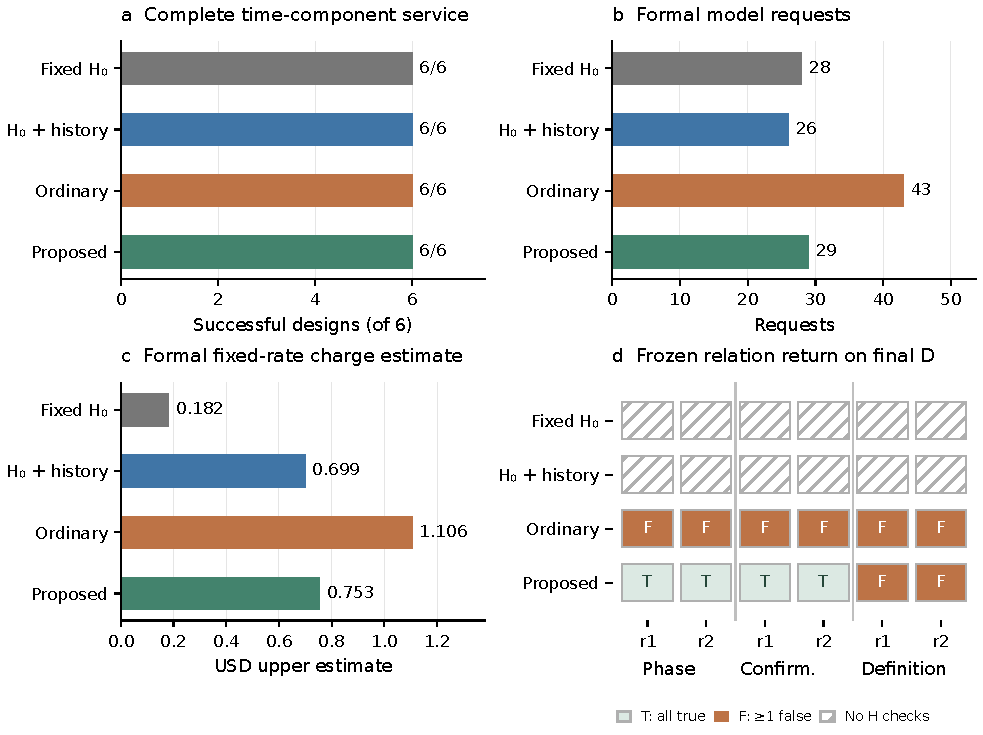
\includegraphics[width=\linewidth]{figures/c24-evidence.pdf}
\caption{The C24 result has three distinct evidence axes. (a) Every arm passes
6/6 complete timing services. (b,c) Formal requests and upper charge estimates
give no proposed-method advantage over equal-history $H_0$. (d) T means every
executed frozen relation returns true on that final design; F means at least
one returns false. Hatched controls submit no learned relation set. All cells
in (d) still have service PASS. These are exact finite observations, with one
method formation per reflection arm; no confidence intervals or population
claim are implied. False relations may flag scope or conservative constraints
and are not automatically scientific errors.}\label{fig:c24}
\end{figure}

\begin{table}[htbp]
\centering\small
\begin{tabular}{@{}lrrl@{}}
\toprule
Stage & Requests & USD upper & Independent result \\
\midrule
Ordinary formation & 4 & 0.1072422 & Structural admission \\
Proposed formation & 6 & 0.1660608 & Structural admission \\
Ordinary validation & 7 & 0.1832448 & Design PASS \\
Proposed validation & 5 & 0.1389699 & Design PASS \\
Proposed first use & 5 & 0.1198866 & Design PASS \\
\midrule
Formal transfer only & 126 & 2.7393975 & 24/24 design PASS \\
All 29 C episodes & 153 & 3.4548018 & No missing usage \\
\bottomrule
\end{tabular}
\caption{C learning and execution costs, charged once per actual episode. Both methods are carried unchanged into final use; validation is not an outcome-based selection gate. The first-use episode belongs only to the proposed arm and is excluded from C24. USD values use frozen token rates and are not invoices.}\label{tab:cstages}
\end{table}

The formal batch uses 126 requests and USD 2.7393975. Adding the two formations,
two validations and proposed first use gives 29 actual C episodes, 153 requests
and USD 3.4548018. All linked provider rows settle. The formal entries record
30 digital scientific executions and no exact-input cache reuse; these counts
are distinct from 126 model requests and 24 final designs. Formation has zero
scientific design execution. This saved-data paper preparation adds none.

\subsection{Why successful designs do not settle the methods' semantics}
Six of six ordinary final designs and two of six proposed final designs have
at least one frozen relation returning false (Figure~\ref{fig:c24}d). This is
a report of the original relations, not an automatic count of unsound methods.
A sufficient condition may reject a feasible design, and a domain guard may
correctly reject a task outside its assumptions. An independent design PASS
therefore neither proves the method nor, by itself, disproves every failed
relation. The artifact's prose and falsifier must also be read against its
declared direction of implication and domain.

For ordinary phase-r1, the design uses a 20 ms period, zero phase,
confirmation-poll origin and $-10$ ms offset. It passes all three service gates,
yet \texttt{centered\_sampling\_budget} and
\texttt{offset\_matches\_centering} return false for both event kinds. The
same two checks return false in confirmation-r1, despite design success.
The frozen qualified-event confirmation/offset prescription is not satisfied
by these participant designs. That discrepancy remains visible; success does
not overwrite the relation returns or establish the prescription's necessity.

For proposed definition-r1, $D$ uses an 80 ms period, 60 ms phase,
\texttt{first\_sample} origin and $-40$ ms offset. Event matching, timely
reception and timestamp accuracy all pass. Nevertheless,
\nolinkurl{event_time_definition_is_qualification} and
\nolinkurl{origin_clock_quantum_budget_within_tolerance} return false on
both start and stop. The task defines event time as onset, so the first false
may be a legitimate scope warning. In definition-r2, only that guard is false.
These results do not confirm transfer of all qualified-event clauses to onset
semantics. They demonstrate successful design execution alongside an unresolved
method-domain boundary.

The study has no independent repeated $H$ formations, clause ablation,
significance test or new hardware family. The three task conditions are finite
and every baseline succeeds, limiting sensitivity to a method gain. The
appropriate outcome is a negative improvement result on this registered
comparison, accompanied by an explicit record of what the frozen relations
did and did not accept. No $G$ expansion or recursive self-improvement follows.
